\subsection{Worker f�r Datenaktualisierung}\label{subsec:Worker}
Gem�� der Abbildung \ref{wissenserwerbskomponente} stellt die Datenverarbeitungskomponente ein Bindeglied zwischen der Wissensbasis (hier Git-Repository) und den Wissenserfassungsverfahren (z.B. Wissenstr�gerschnittstelle) dar. Auf Implementierung bezogen handelt es sich um ein Programm, das f�r eine kleine Aufgabe zust�ndig ist. Martin Flowler bezeichnet das als Mircoservice\footnote{https://www.martinfowler.com/articles/microservices.html}. Im Fall von \textit{PaaSfinder} wird dieser Microservice als \glqq{}Worker\grqq{} bezeichnet. Schematisch wird der Worker in Abbildung \ref{fig:worker} dargestellt.
\begin{figure}[H] 
	\centering
	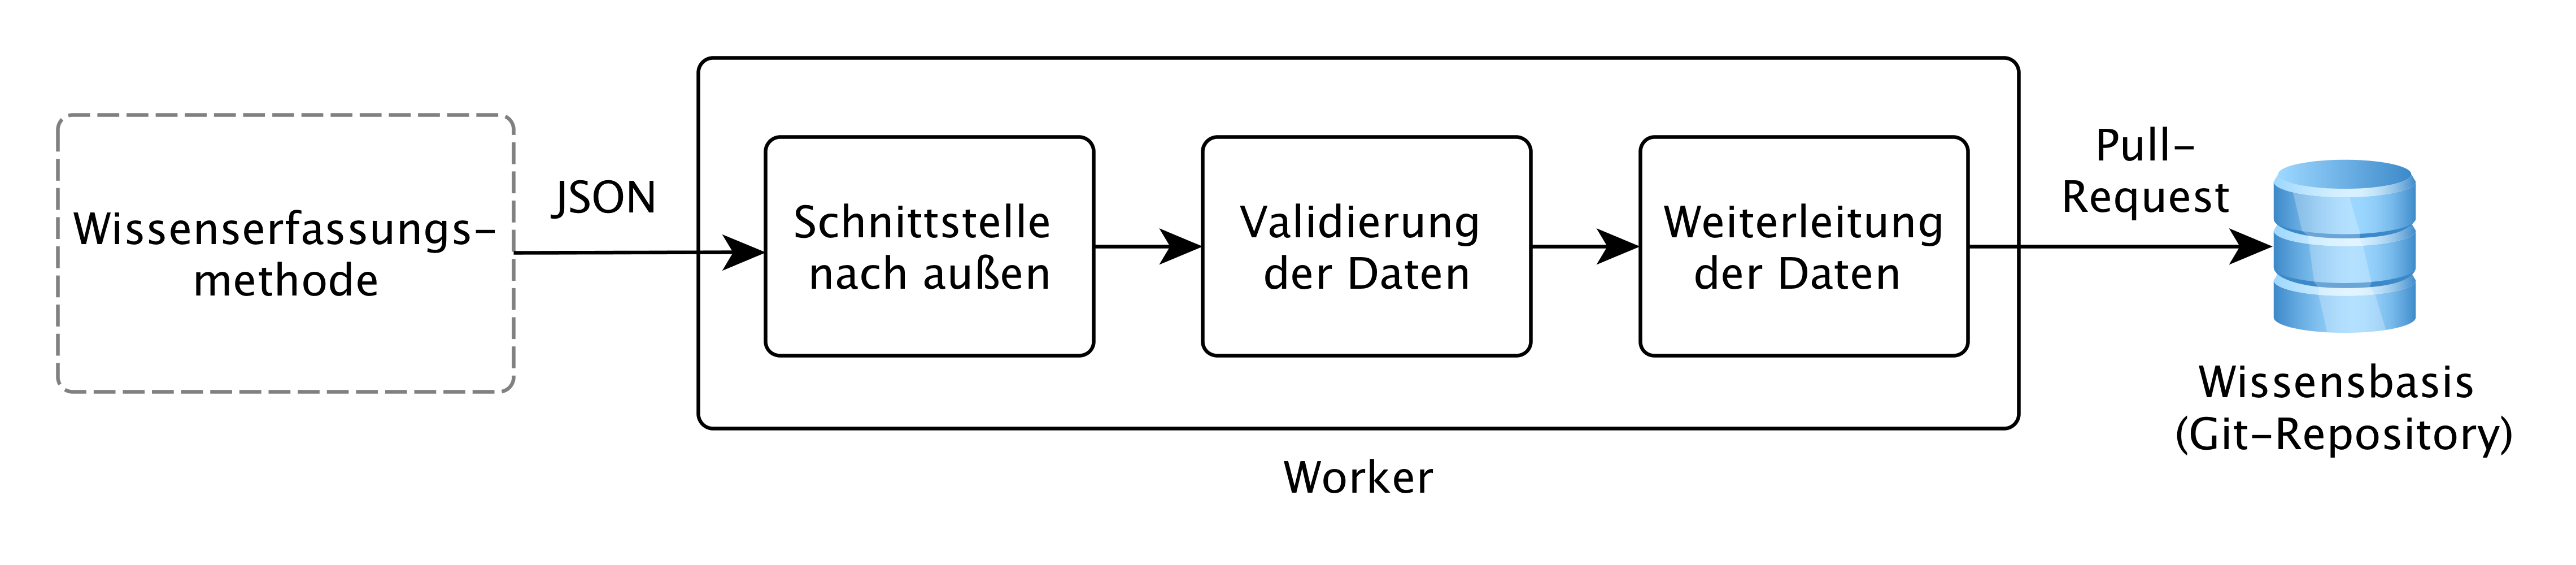
\includegraphics[width=1.0\textwidth]{images/worker.png}
	\caption{Der Aufgabenbereich vom Worker}
	\label{fig:worker}
\end{figure}
Der Aufgabenbereich vom Worker ist einfach. Zun�chst sollen die Daten durch eine Schnittstelle empfangen werden.  Dabei wird der Ausschlusskriterium angewandt, dass nur die Daten in JSON Format akzeptiert werden. Sobald die Daten vorliegen, werden sie im n�chste Schritt entsprechend f�r das Senden vorbereitet und an die Wissensbasis weitergegeben. In diesem Fall handelt es sich um die Erstellung eines Pull-Requests, der anschlie�emd an die Git-Repository gesendet wird.\\
Die allgemeine Architektur des Workers basiert auf \ac{REST}-Stil, der urspr�nglich aus der Dissertation von Fielding \cite{fielding2000} stammt. Das zentrale Konzept von REST sind Ressourcen \cite[S.35]{tilkov2015}. In diesem Fall sind das aktualisierte JSON-Objekte eines PaaS-Profils, die an die REST-Schnittstelle gesendet werden. Tilkov et al. \cite{tilkov2015} beschreiben REST durch folgende Grundprinzipien:
\begin{itemize}
\item Ressourcen mit eindeutiger Identifikation
\item Verkn�pfung/Hypermedia
\item Standardmethoden
\item Unterschiedliche Repr�sentationen
\item Statuslose (stateless) Kommunikation
\end{itemize}